\chapter{Internship Activities and Project Work}
\label{ch:activities}

This chapter is the heart of the report. It describes what I actually
did at FlowGenX AI during my five-and-a-half-month internship: who I
worked with, how I onboarded, what I learned in the early weeks, and
the specific live-product contributions I made between November 2025
and May 2026. The chapter is organised into two phases, mirroring
the natural arc of my internship: an initial learning period followed
by sustained live-project work on the company's connectivity layer.

\section{Overview of My Role}
I joined FlowGenX AI on \textbf{10 November 2025} in the position of
\emph{Full Stack Software Engineer -- Generative AI (Intern)}, and
worked full-time, remotely from Bangladesh, until \textbf{02 May 2026}.
This was a tenure of approximately five and a half months ---
exceeding the four-month minimum stated in my offer letter --- during
which I was integrated into the company's \emph{connectivity team}.

\subsection{The Connectivity Team}
The team I joined is responsible for the FlowGenX platform's
integration substrate: the framework, the connector catalogue, and
all the supporting tooling that exposes external services to the
runtime, the workflow engine, and ultimately the end user.

The people I worked with most closely on a daily basis were:

\begin{itemize}[leftmargin=*]
    \item \textbf{Mr.~Sanjib Sen} --- Senior Software Engineer and
    Team Lead. Sanjib bhai owns the architectural direction of the
    connectivity layer and is the senior reviewer for non-trivial
    changes.
    \item \textbf{Mr.~Abrar Bin Rofique} --- Software Engineer
    (Generative AI), my direct supervisor. Abrar bhai owned my
    onboarding, the day-to-day technical guidance, and the bulk of
    the code review on my pull requests.
    \item \textbf{Mr.~Ashikuzzaman Abir} --- Software Engineer,
    additional mentor. Ashik bhai supports the workflow-agent side of
    the platform, and he was the person I went to whenever my
    connector work touched the workflow runtime --- helping me
    understand how a connector method becomes a callable node inside
    a real end-to-end agent workflow.
    \item \textbf{Mr.~Nayem Islam} --- Software Engineer / AI
    Engineer working closely with the connectivity team.
    \item \textbf{Mr.~Latiful Kabir} --- Software Engineer
    (Generative AI), also working closely with the connectivity team.
\end{itemize}

I was the only intern on the team for the duration of my engagement
and was treated as a contributing member rather than a learner-only,
in keeping with the company-wide culture of valuing impact over
titles.

\subsection{The Primary Project}
My primary project was the \texttt{runtime\_connectivity} repository
--- FlowGenX AI's unified Python framework for connecting the platform
to external systems. By the end of my internship I had authored
\textbf{178 commits} across the \texttt{dev} branch and dozens of
feature branches, and delivered \textbf{more than ninety
production-ready connectors} to the platform's integration catalogue.

\section{Phase One: Initial Learning Period (Weeks 1--2)}
The first two weeks of my internship were a deliberate ramp-up
period. The work in this phase was not merely tutorial-style learning;
the very first connectors I built (Weaviate, Discord, Notion, and a
fix to Google Chat) shipped to production. The intent of the phase
was to learn the framework by building inside it.

\subsection{Setting Up the Development Environment}
The very first task was to bring up a working local development
environment for the connectivity package and the surrounding runtime
services. This involved:

\begin{itemize}[leftmargin=*]
    \item Installing Python 3.11 and the \texttt{uv} package manager.
    \item Cloning the four repositories
    (\texttt{flowgenx-nextjs-V2}, \texttt{runtime\_apis},
    \texttt{runtime\_components}, \texttt{runtime\_connectivity}) into
    a shared parent directory so that local editable installs could
    cross-reference each other.
    \item Running \texttt{uv pip install -e ".[dev]"} inside
    \texttt{runtime\_connectivity} to install the package in editable
    mode along with all developer dependencies.
    \item Installing the \texttt{pre-commit} hooks so that every
    commit I made would be automatically formatted and linted.
    \item Configuring a local PostgreSQL instance and Docker Desktop
    on Windows for connector testing and end-to-end integration runs.
    \item Standing up the FastAPI service through the project's
    \texttt{dev.sh up} script and verifying that the Swagger UI
    (\texttt{http://localhost:8081/docs}) and the Airflow UI
    (\texttt{http://localhost:8080}) were both reachable.
\end{itemize}

\subsection{Understanding the Connector Framework}
Before writing my first connector, my supervisor walked me through
the project's three-tier abstraction
(\texttt{BaseManager} → \texttt{DBManager}/\texttt{FSManager}/%
\texttt{ObjManager}), the \texttt{@openapi\_endpoint} decorator, the
dual sync/async pattern, the \texttt{ConnParams} convention, and the
metadata-generation pipeline that takes a connector from source code
to UI. I read the project's internal documentation end-to-end, then
reverse-engineered an existing connector
(PostgreSQL) to see how all the pieces fit together in practice.

The most important conceptual insight from this period was that a
connector at FlowGenX is not just a Python class; it is a
\emph{four-artefact bundle}:

\begin{enumerate}[leftmargin=*]
    \item Source code (\texttt{ConnParams} + \texttt{Manager} +
    per-method modules, decorated with OpenAPI metadata).
    \item Integration tests (\texttt{test\_<name>\_connector.py}).
    \item Auto-generated metadata
    (\texttt{openapi\_spec.json}, \texttt{auth\_config.json},
    \texttt{connector\_metadata.json}).
    \item A UI Endpoint Test Reference document for end users.
\end{enumerate}

Internalising this four-artefact contract was what made my work
self-consistent from the very first connector onwards.

\subsection{First Connectors as Learning Artefacts}
With my environment set up and the framework understood, the second
half of the onboarding period was hands-on. Between
\textbf{20 November and 30 November 2025} I shipped my first
production connectors:

\begin{itemize}[leftmargin=*]
    \item \textbf{Weaviate} --- a vector-database connector. This was
    my first end-to-end implementation. Building it taught me how to
    model schema-less data, work with vector embeddings, and write
    the \texttt{near\_vector} similarity-search method.
    \item \textbf{Discord} --- a messaging-platform connector that
    taught me how OAuth-style bearer tokens work in practice.
    \item \textbf{Notion} --- a productivity-tool connector. This is
    where I first wired up environment-variable support and applied
    the \texttt{@openapi\_endpoint} decorator end-to-end.
    \item \textbf{Perplexity AI} --- my first AI-provider connector.
    \item \textbf{QuickBooks (initial scaffolding)},
    \textbf{Uber}, \textbf{Shopify}, \textbf{S\&P Global},
    \textbf{ClickUp}, \textbf{MongoDB}, and an initial
    \textbf{Stripe} connector --- each one teaching me a slightly
    different aspect of authentication, pagination, or
    error handling.
    \item A \textbf{Google Chat fix} --- my first real
    bug-fix-and-merge experience inside someone else's connector.
\end{itemize}

By the end of week two I had merged my first half-dozen pull requests
and had a complete mental model of the codebase. Phase one was
complete; phase two could begin.

\section{Phase Two: Live Project Involvement}
The remaining five months of the internship were spent contributing
to \texttt{runtime\_connectivity} as a normal team member. The work
fell into four categories: \textbf{feature development} (new
connectors), \textbf{bug fixes and reliability work}, \textbf{code
improvement and refactoring}, and \textbf{documentation}. I describe
each in turn, then narrate a few of the most substantial connectors
in greater depth.

\subsection{The Connector Lifecycle in Practice}
Every connector I delivered followed the same eleven-step lifecycle.
\textbf{(1) API research} --- read the third-party documentation and
identify the auth model, priority methods, pagination, rate limits,
and quirks. \textbf{(2) Branch} the feature off \texttt{dev}.
\textbf{(3) Connection-parameter modelling} --- define a
\texttt{ConnParams} Pydantic model with the right field types,
descriptions, and \texttt{json\_schema\_extra} UI metadata.
\textbf{(4) Manager class} --- subclass the appropriate base manager
(\texttt{DBManager}, \texttt{FSManager}, or \texttt{ObjManager}) and
implement \texttt{\_connect}, \texttt{\_close}, and
\texttt{test\_connection}. \textbf{(5) Per-method modules} ---
implement each business method in its own file, decorated with
\texttt{@openapi\_endpoint}, using the dual sync/async helpers.
\textbf{(6) Integration test script} ---
\texttt{test\_<connector>\_connector.py} hits the live API with
real credentials and produces a
\textsc{PASS}\,/\textsc{FAIL}\,/\textsc{SKIP} report per endpoint.
\textbf{(7) Sample backfill} --- capture real request and response
payloads from the integration run and embed them as the decorator's
\texttt{example} and \texttt{response\_sample} values.
\textbf{(8) Metadata generation} --- run
\texttt{generate\_openapi\_spec.py},
\texttt{generate\_auth\_config.py}, and
\texttt{populate\_connector\_db.py} so the connector becomes
visible in the UI. \textbf{(9) Pull request and review} ---
descriptive \texttt{feature/Rakib/(<connector>): <summary>} commit,
review cycle, merge into \texttt{dev}.
\textbf{(10) Endpoint testing} after merge through the API tester,
the MCP Playground (Figure \ref{fig:mcp-playground}), and an
end-to-end workflow run (Figure \ref{fig:workflow-editor}); update
the ClickUp card. \textbf{(11) Documentation} --- for high-value
connectors, author a \emph{UI Endpoint Test Reference} cookbook.
Internalising and operating this lifecycle cleanly was the single
most important habit I built during the internship.

\begin{figure}[H]
    \centering
    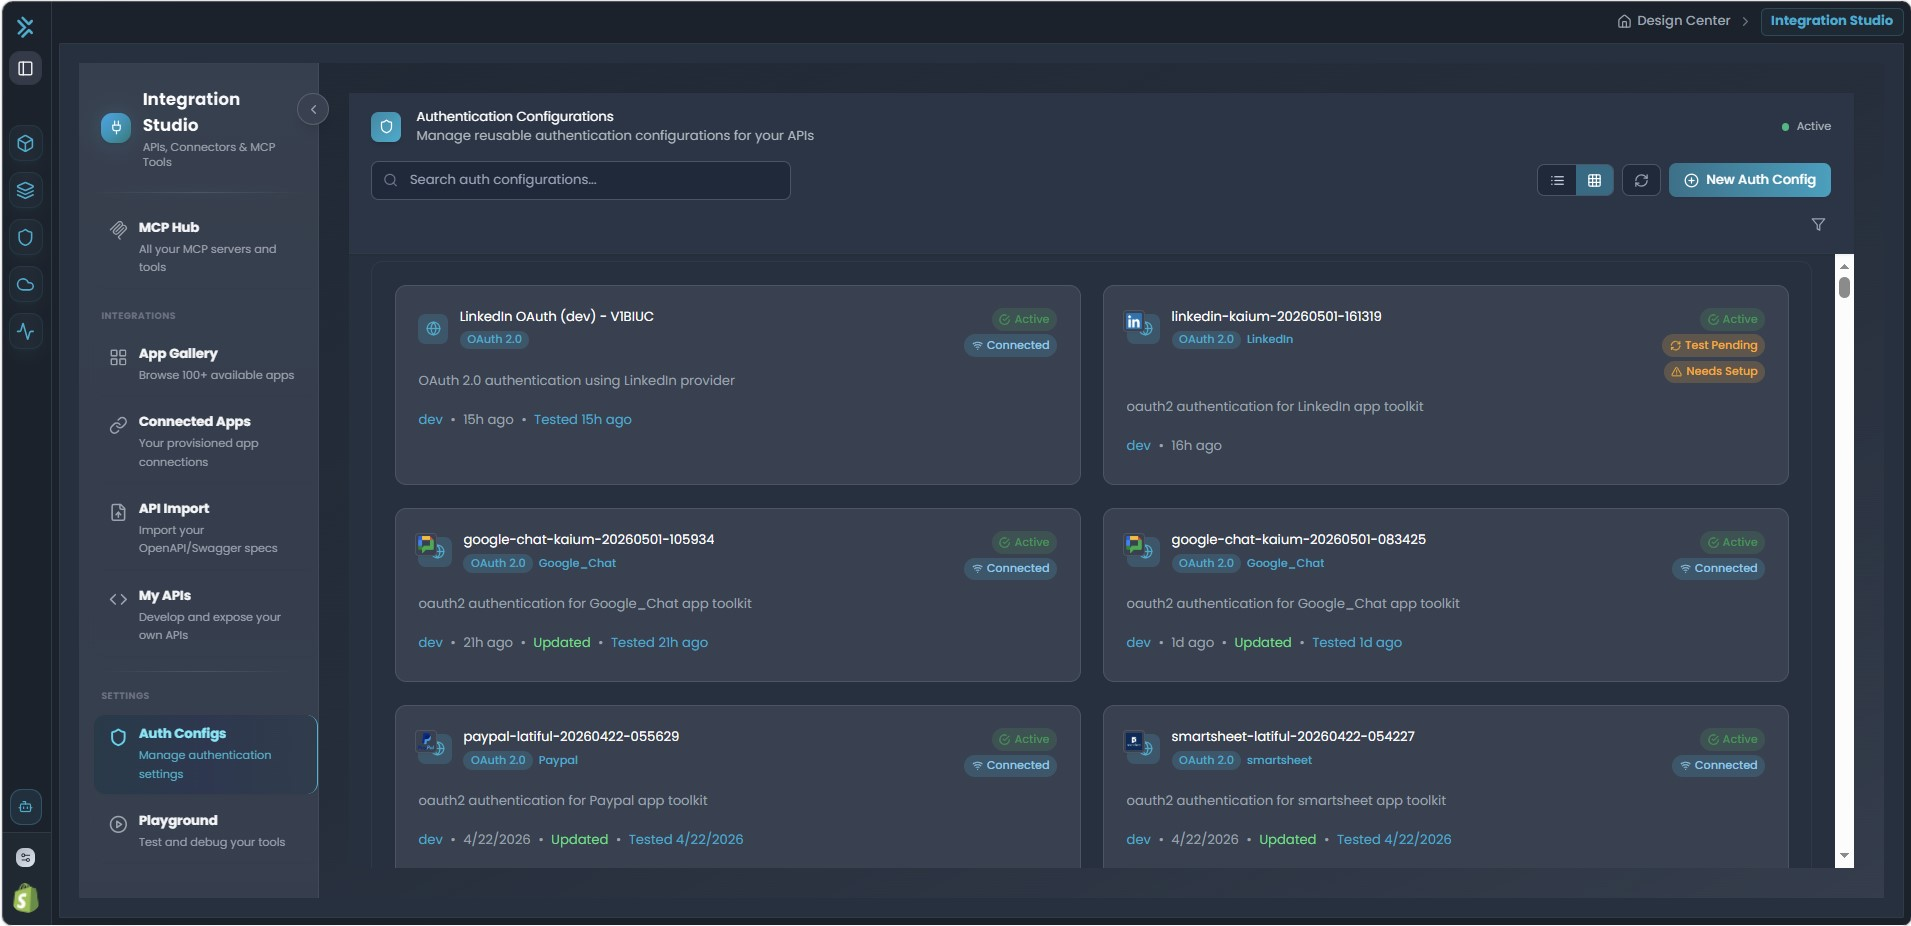
\includegraphics[width=0.8\textwidth]{figures/screenshots/Auth_config.jpg}
    \caption{Authentication configuration page driven by
    \texttt{auth\_config.json}.}
    \label{fig:auth-config}
\end{figure}

\subsection{Work Timeline}
Table \ref{tab:work-timeline} summarises what I delivered across
the twenty-four weeks of the internship. The table is compiled
directly from my Git history on the \texttt{runtime\_connectivity}
repository.

\begin{table}[H]
\centering
\renewcommand{\arraystretch}{1.25}
\begin{tabularx}{\textwidth}{l X}
\toprule
\textbf{Period} & \textbf{Connectors and work delivered} \\
\midrule
Nov 20 -- Nov 30, 2025 & Weaviate; Discord; Notion (full setup with env-var support and decorators); Perplexity AI; QuickBooks (initial); Uber; Shopify (test pass); Google Chat fix; S\&P Global; ClickUp; MongoDB; Stripe (initial). \\
\addlinespace
Dec 1 -- Dec 14, 2025 & Elasticsearch (with Windows encoding fix); Datadog; Milvus; LaunchDarkly; Zoho CRM; FreshDesk; Yelp; Stripe; FreshBooks; Xero; GitLab; GitHub; Zoho Desk; Apollo.io; Zoom; WordPress; Customer.io; BambooHR; Lever; OneDrive; SharePoint; FreshBooks endpoint refactor. \\
\addlinespace
Dec 15 -- Dec 31, 2025 & AWS S3 (bucket policies, versioning, multipart uploads); MySQL upgrades (truncate / update / upsert); PostgreSQL enhancements; Pinecone; Tavily; Exa; SerpAPI; AWS RDS PostgreSQL; AWS RDS MySQL; dbt-cloud; OpenWeatherMap; Freshsales; Zendesk Sell; Auth0; Massive; MSSQL with full CRUD; Azure Blob Storage; Azure SQL Server (firewall + retry); Groq; OpenAI. \\
\addlinespace
Jan 1 -- Jan 15, 2026 & Anthropic (with Files / Skills API restructure); DeepSeek; xAI; Azure Data Lake; Typesense; X (Twitter); LINE Messaging; Google Tasks; GitHub Actions; Google Forms; Gusto; Zoho Inventory; Zoho Books. \\
\addlinespace
Jan 16 -- Jan 31, 2026 & Zoho Analytics (User Management + data manipulation); Zoho Campaigns; Mailchimp; EPIC FHIR (initial groundwork and permissioning); Microsoft Dynamics 365 Business Central; Linear; AlphaSense; Gong; Outreach; 6sense; SalesLoft; Rippling; FactSet; Google Chat. \\
\addlinespace
Feb 1 -- Feb 28, 2026 & Jira Service Management; Typeform; Ashby; Freshservice; Okta; Crunchbase; HelpScout; AWS Textract (23 methods, sync + async + adapters); AWS Rekognition (75 methods covering image, video, face, custom labels, stream processors); HelpScout UI test-reference doc; Rekognition endpoint test reference. \\
\addlinespace
Mar 1 -- Mar 15, 2026 & Octagon (15 financial-research agents); Harness (46 methods across V1 + legacy APIs); SonarQube (34 methods across server + cloud); QuickBooks access-token refresh; QuickBooks OAuth callback fix; Typesense OpenAPI spec; OpenAI / Exa / SerpAPI / Stripe UI Endpoint Test Reference docs; Google Forms enhancements. \\
\addlinespace
Mar 16 -- Mar 31, 2026 & OpenFIGI (4 methods, API key auth); Notion UI test reference; GitHub \texttt{write\_object\_to\_dataframe} refactor (list support); AWS RDS MySQL registry registration; Supabase (50 methods); Eventbrite; Google Meet; Apify (69 methods, webhook + wait-for-run). \\
\addlinespace
Apr 1 -- Apr 15, 2026 & Attio; Instantly (63 methods); Chorus; NeverBounce; PostgreSQL parameter standardisation; LinkedIn Sales Navigator (with token refresh); MySQL connector list/DataFrame support; ClickUp response-sample backfill. \\
\addlinespace
Apr 16 -- May 2, 2026 & Documentation pass and polish: GitLab API doc + response samples; Freshsales API enhancements; Mailchimp test + doc updates; FreshDesk doc enhancements; Freshservice integration scripts + endpoint test reference; Freshworks CRUD enhancements; Zoho CRM UI test reference; Zoho Analytics UI test reference; Zoho Campaigns final polish. \\
\bottomrule
\end{tabularx}
\caption{Connectors and work delivered, week by week, on the
\texttt{runtime\_connectivity} repository.}
\label{tab:work-timeline}
\end{table}

Figure \ref{fig:app-gallery} shows how connectors appear in the
FlowGenX application gallery, and Figure \ref{fig:connected-apps}
shows the connected-apps page where end users manage their live
authentications. The full categorical breakdown of the integration
catalogue is given in Section~\ref{sec:integration-catalogue} and
need not be repeated here.

\begin{figure}[H]
    \centering
    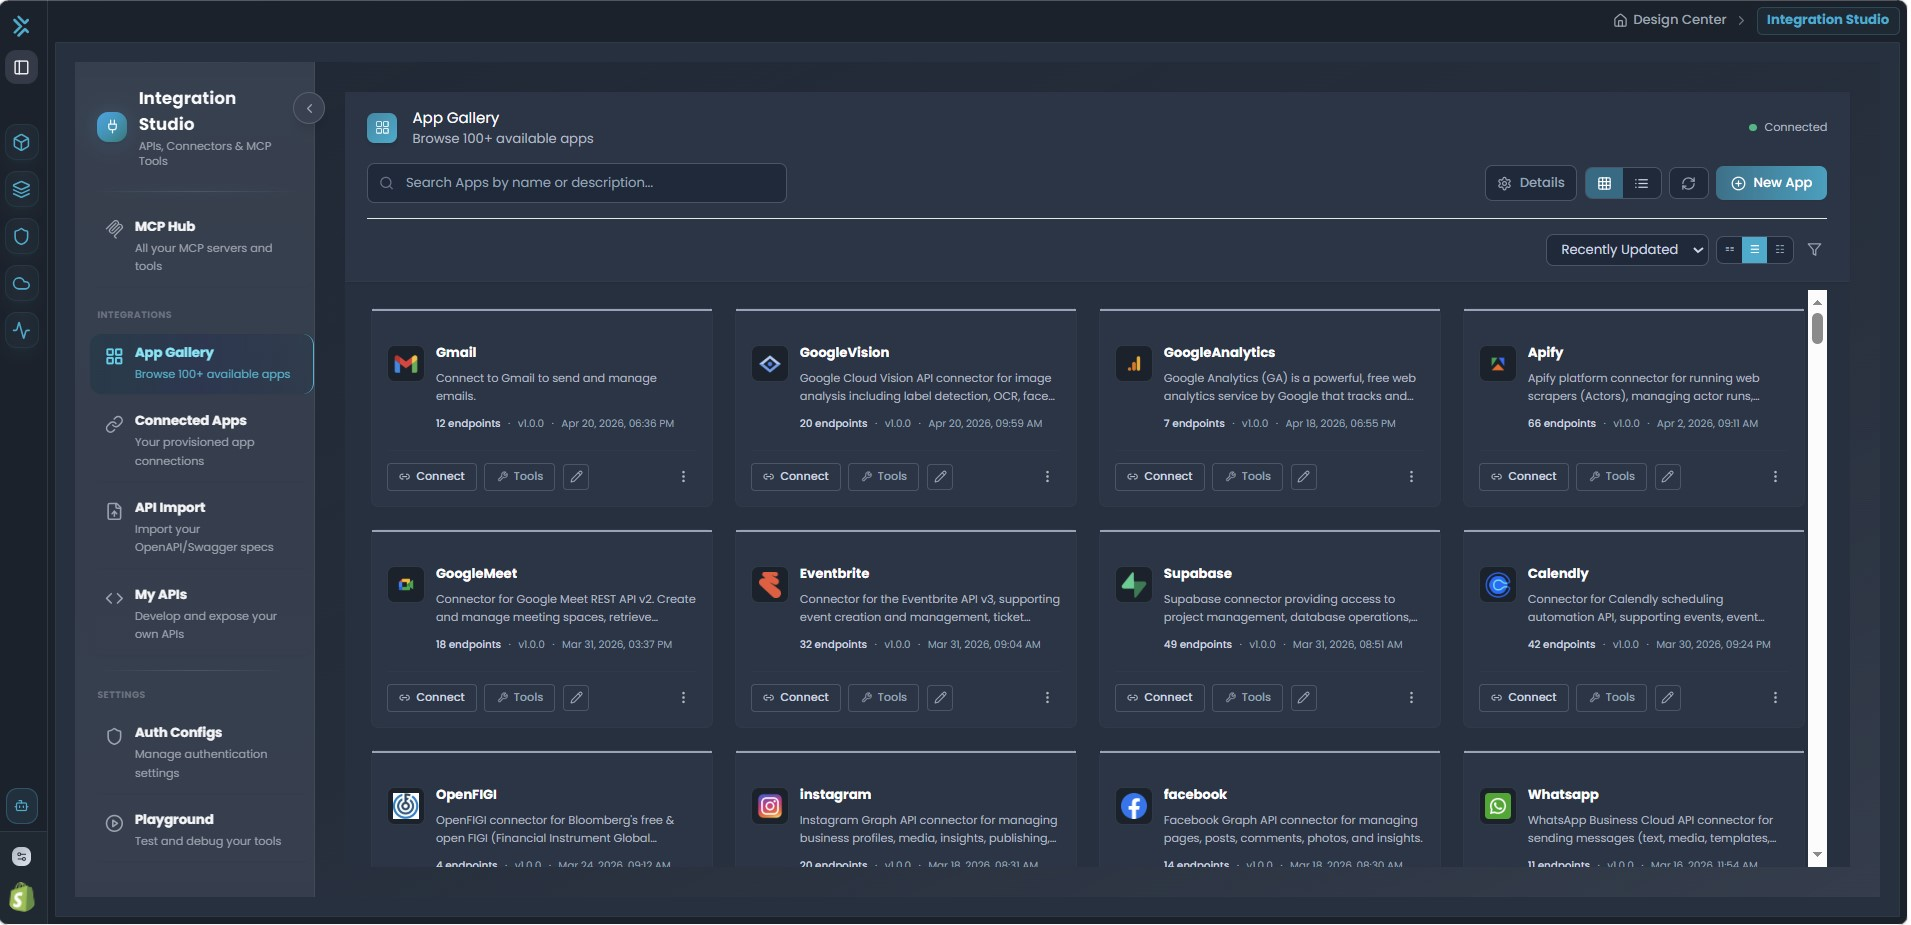
\includegraphics[width=0.8\textwidth]{figures/screenshots/APP_gallery.jpg}
    \caption{The FlowGenX AI app gallery, populated by connectors
    delivered through \texttt{runtime\_connectivity}.}
    \label{fig:app-gallery}
\end{figure}

\begin{figure}[H]
    \centering
    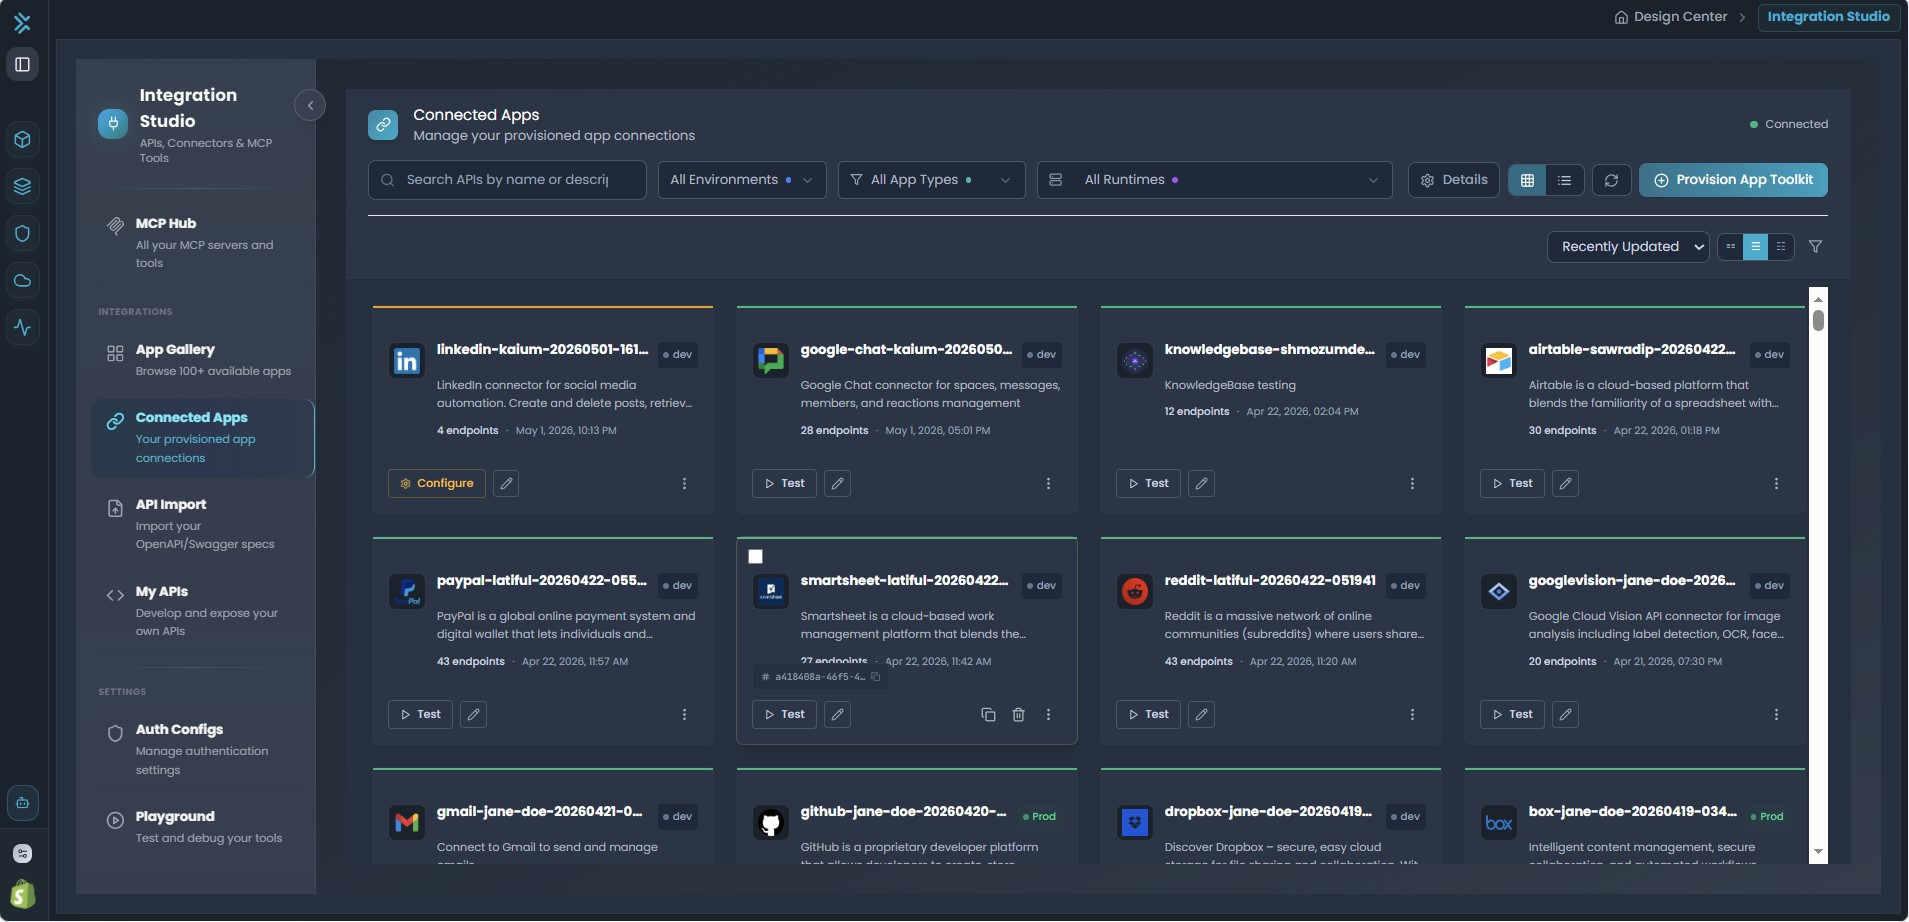
\includegraphics[width=0.8\textwidth]{figures/screenshots/Connected_apps.jpg}
    \caption{End-user view of connected apps (active authentications)
    on the FlowGenX platform.}
    \label{fig:connected-apps}
\end{figure}

\section{Bug Fixes and Reliability Work}
Alongside new feature delivery I shipped a number of reliability
improvements. The most consequential were the \textbf{OAuth2
redirect-URI fixes} for QuickBooks and FreshBooks --- the QuickBooks
fix shipped together with an \emph{access-token refresh mechanism}
so that long-running sessions stopped failing with 401 errors --- the
\textbf{SQL Server retry logic} added to stabilise flaky connection
tests under transient network errors (plus a firewall-rule
mode-selection enhancement for Azure SQL Server), and the
\textbf{Windows console encoding fix} in the Elasticsearch connector
that prevented a Unicode crash on the Windows test runner and
unblocked the Windows-based developers on the team. Smaller but
production-relevant fixes included WordPress connector hardening
(\texttt{list\_blocks} error handling, malformed base-URL
construction in \texttt{search\_content}), the Customer.io test
configuration fix for an outdated API key, the Google Chat
post-method malformed-request-body fix, a cache-cleanup fix that
prevented stale data between connector test runs, Datadog
log-ingestion debugging, AWS RDS MySQL registry registration, and
GitLab revert coordination after a teammate's revert.

\section{Code Improvement and Refactoring}
Reliability and feature work were complemented by a handful of
larger refactors. The most impactful was the \textbf{DataFrame /
list duality across SQL connectors} --- standardising parameter
naming and accepted shapes across PostgreSQL, MySQL, and GitHub so
that write methods transparently accept either a
\texttt{pandas.DataFrame} or a plain \texttt{list[dict]}, which
made the connectors significantly more flexible for downstream
consumers that did not always have pandas in scope. The
\textbf{AWS Textract} and \textbf{Anthropic} connectors were both
restructured to separate sync and async document-analysis methods
and to cleanly split the Files API from the new Skills API
respectively. Smaller refactors included the \texttt{Zoho\_CRM}
folder rename to align with project casing conventions, an
improved LaunchDarkly test script with cleanup logic and richer
logging, and general readability passes on the FreshBooks endpoints
(clients, expenses, invoices, tasks, time entries) and other
resource-heavy connectors. Finally, the \textbf{OpenAPI sample
backfill} replaced placeholder values in \texttt{request\_schema}
and \texttt{response\_sample} with real values captured from live
API runs (FreshDesk, Freshservice, GitLab, ClickUp, Apify, Instantly,
Mailchimp, Freshsales, Freshworks, and others) --- the work that
directly improves the end-user experience by pre-filling forms with
values that actually work.

\section{Documentation Contributions}
A connector at FlowGenX is not considered fully complete until it has
a UI Endpoint Test Reference document --- a concrete, hands-on
cookbook that shows end users how to call each method from the
platform UI, what parameters to provide, and what shape of response
to expect. I authored such documents for many of the high-value
connectors I delivered, including Notion, Stripe, OpenAI, Exa,
SerpAPI, HelpScout, Typesense, Zoho CRM, Zoho Analytics, Zoho
Campaigns, FreshDesk, Freshservice, AWS Rekognition, and Google
Forms. These documents serve a dual purpose: they give end users
immediate clarity on how to use a connector, and they give other
engineers a ready-made test plan when they need to verify that a
connector still works after an upstream API change.

\begin{figure}[H]
    \centering
    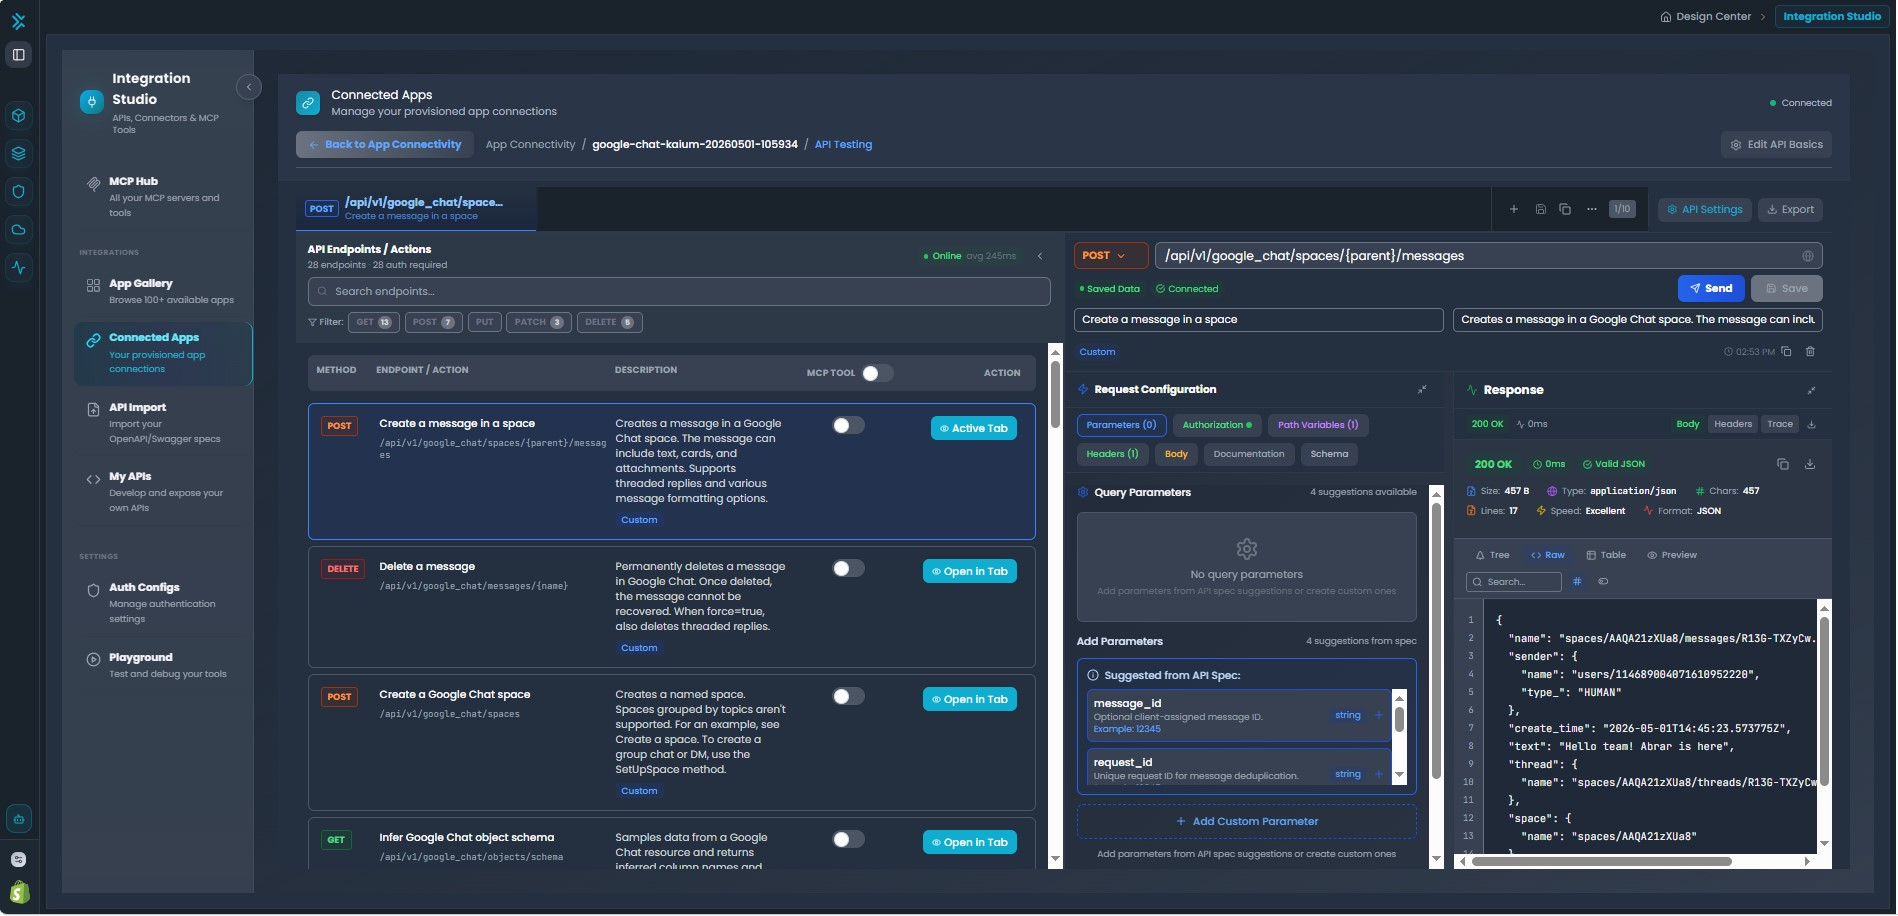
\includegraphics[width=0.8\textwidth]{figures/screenshots/paricular_connector_endpoint_test.jpg}
    \caption{Per-connector endpoint testing UI used during validation.}
    \label{fig:endpoint-test}
\end{figure}

\section{Collaboration and Workflow Discipline}
Across the entire engagement, the way I worked with the rest of the
team mattered as much as the code I shipped. Each connector was
developed on its own feature branch (\texttt{wordpress-connector},
\texttt{Harness\_connector}, \texttt{MySQL-connector},
\texttt{Google-Forms-connector}, and so on); \texttt{dev} was the
integration branch and was never committed to directly. Every commit
followed the convention
\texttt{feature/Rakib/(<connector>): <summary>}, so reviewers could
trace work per integration without reading diffs. Feature branches
were kept up-to-date with \texttt{origin/dev}, with non-trivial
manual merges on the AWS Textract, HelpScout, X (Twitter), Harness,
Google Forms, FreshBooks, Freshworks, and Zoho CRM branches. Every
merge was paired with a re-run of the metadata pipeline
(\texttt{generate\_openapi\_spec.py},
\texttt{generate\_auth\_config.py},
\texttt{populate\_connector\_db.py}) so the connector appeared in
the FlowGenX UI immediately rather than requiring a follow-up pass.

The internship also gave me room to explore technologies beyond the
strict scope of my connector work --- the \emph{Model Context
Protocol (MCP)} (exercised through the MCP Playground for almost
every connector I shipped), \emph{Agent-to-Agent (A2A)}
communication, gRPC patterns inside \texttt{runtime\_apis}, the
Apache Airflow side of the workflow engine, and the reusable
\texttt{runtime\_components} library (\texttt{FilterComponent},
\texttt{DataMappingComponent}, \texttt{DataPrivacyComponent} with
PII masking, \texttt{JoinerComponent}, \texttt{HTTPNodeComponent},
\texttt{ForeachComponent}, \texttt{SwitchComponent}, and the
\texttt{SensorComponent}). These exposures, although not part of my
shipped pull requests, gave me an end-to-end picture of how an
agentic platform fits together.

\section{Impact in Summary}
Delivered 90+ production-ready connectors and standardised heavy
APIs behind Manager classes, improving reliability (retry logic,
token refresh, encoding and error-handling) and enabling broad
platform operations. I also added real API samples, OpenAPI specs,
and UI test-reference docs to speed adoption and make connectors
easy for teammates to reuse.
